\documentclass{article}

\usepackage{graphicx}
\usepackage{tikz}
\usepackage{tikzsymbols}
\usetikzlibrary{calc,patterns,shapes.geometric}
\pagestyle{empty}
\usepackage[margin=0pt]{geometry}
\geometry{papersize={14in,12in}}

\def\centerarc[#1](#2)(#3:#4:#5){\draw[#1] ($(#2)+({#5*cos(#3)},{#5*sin(#3)})$) arc (#3:#4:#5);}

\begin{document}
	\begin{figure}
		\centering
		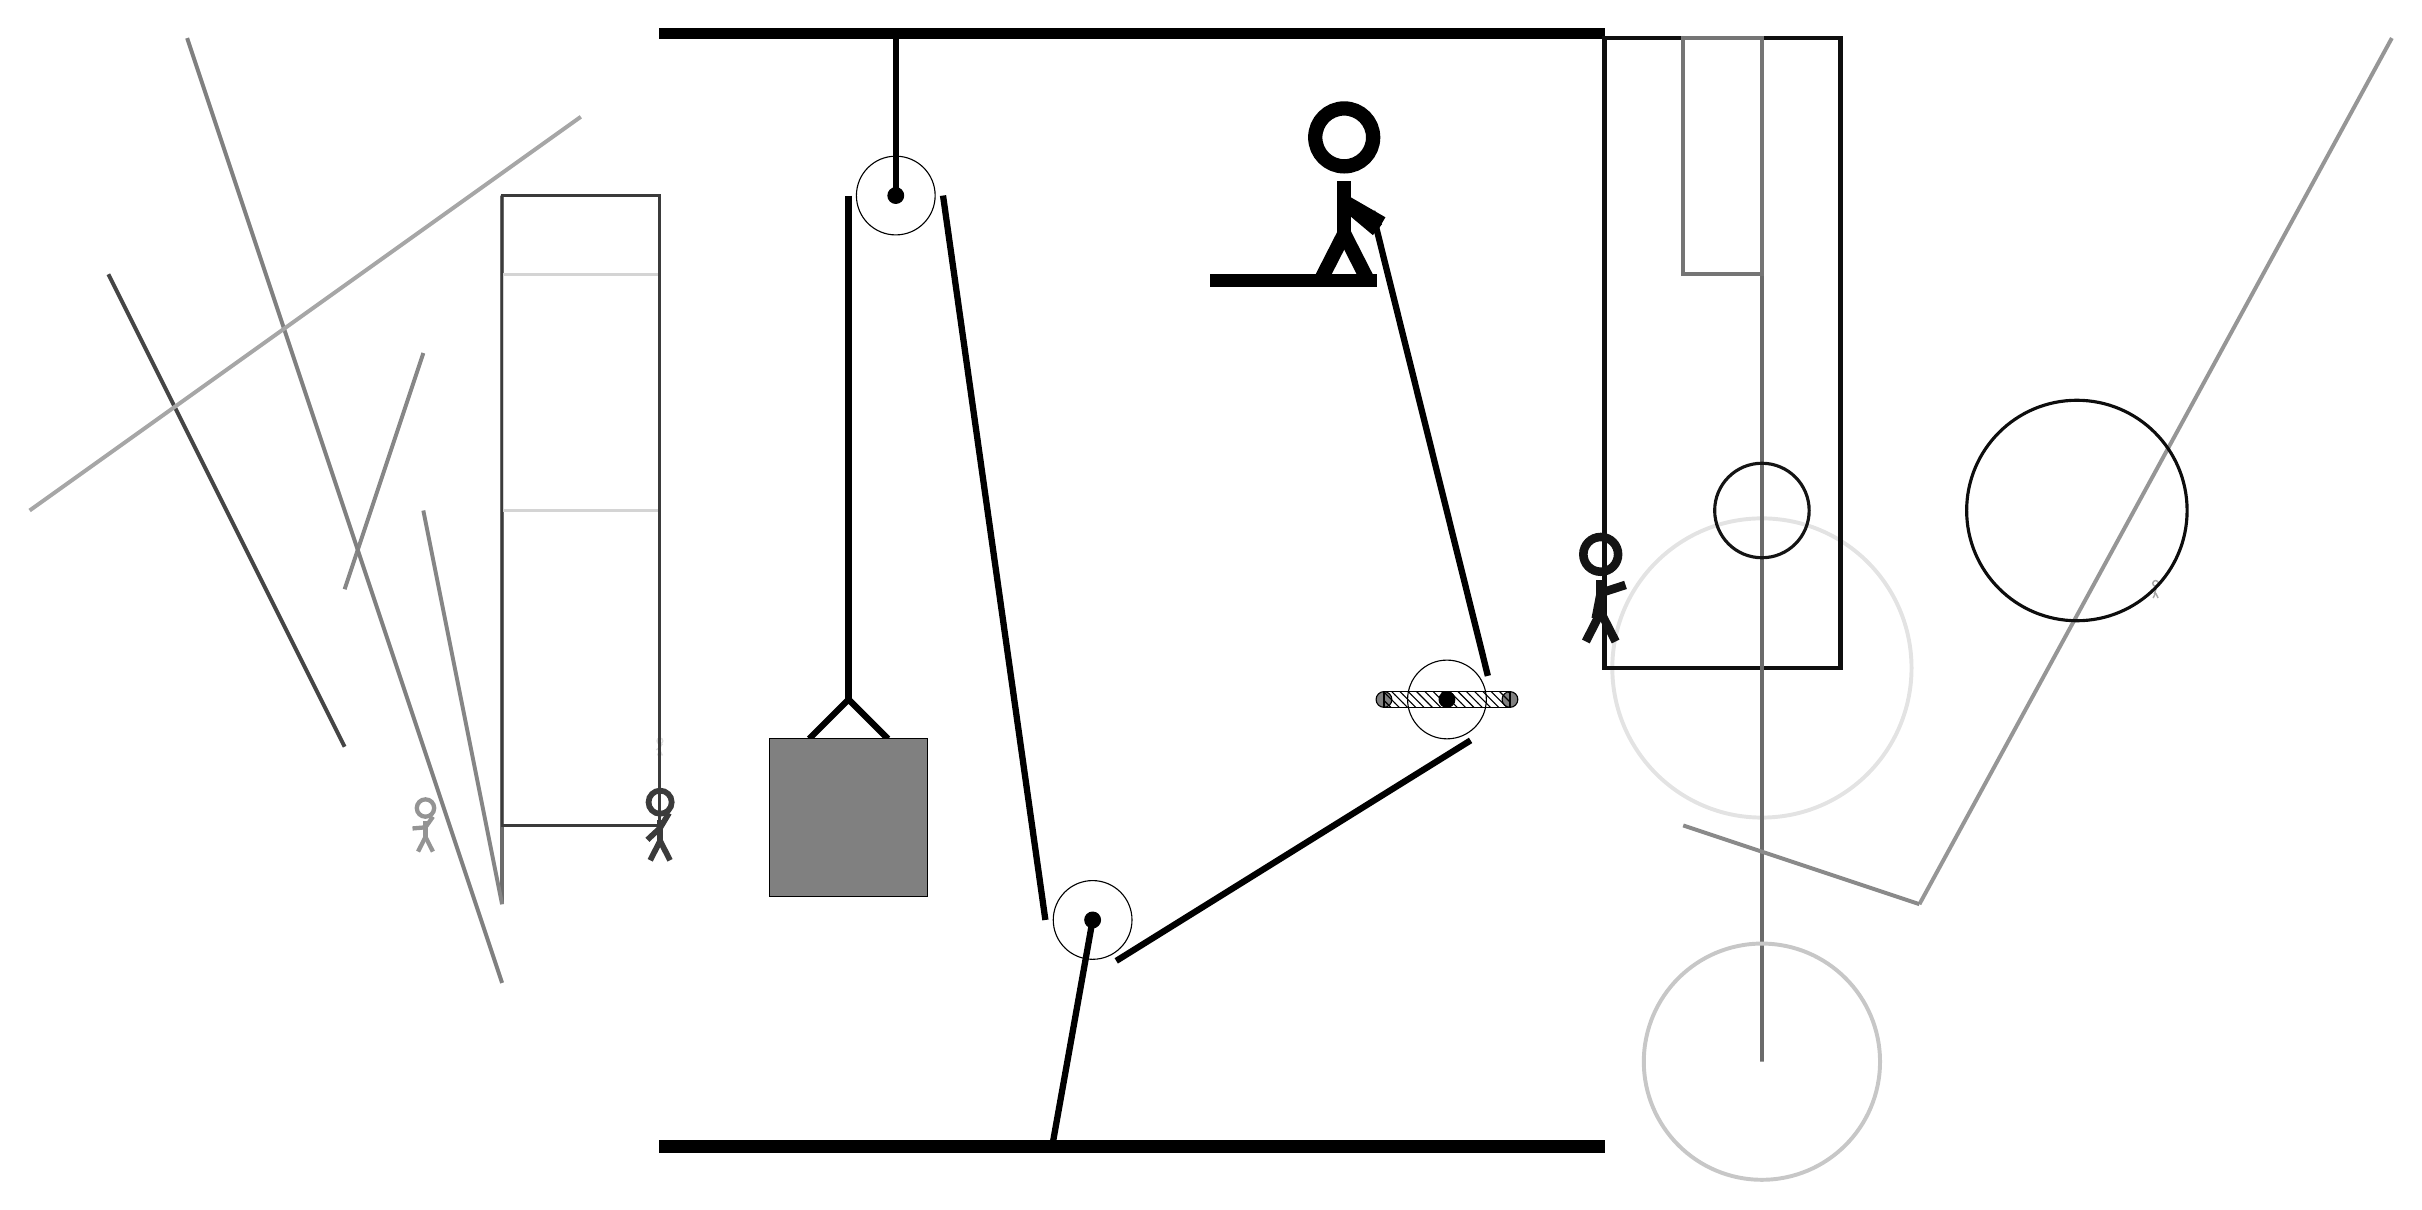
\begin{tikzpicture}
			%%%%% START %%%%%
			
			\draw[fill=black] (-2, 14) rectangle (10, 14.125);
			
			\draw (1, 12) circle (0.5);
			\draw[fill=black] (1, 12) circle (0.1);
			\draw[line width=0.8mm] (1, 14) -- (1, 12);
			
			\draw (3.5, 2.8) circle (0.5);
			\draw[fill=black] (3.5, 2.8) circle (0.1);
			\draw[line width=0.8mm] (3.5, 2.8) -- (3.0, 0);
			
			\draw [line width=0.5mm, color=black!11](12, 6) circle (1.9);
			
			\node[line width=0.4mm, color=black!34] at (17, 7) {\Strichmaxerl[1][71][79]};
			\draw[line width=0.5mm, color=black!58] (-4, 3) rectangle (-4, 12);
			\draw[line width=0.6mm, color=black!94] (10, 6) rectangle (13, 14);
			\node[line width=0.5mm, color=black!13] at (-2, 5) {\Strichmaxerl[1][35][55]};
			\draw[line width=0.5mm, color=black!73](-6, 5) -- (-9, 11);
			\draw [line width=0.4mm, color=black!72](-3, 4) circle (0.0);
			\draw[line width=0.4mm, color=black!17] (-4, 8) rectangle (-2, 11);
			\node[line width=0.7mm, color=black!77] at (-2, 4) {\Strichmaxerl[4][43][59]};
			\draw[line width=0.4mm, color=black!58] (12, 11) rectangle (12, 1);
			\draw[line width=0.5mm, color=black!47](-5, 10) -- (-6, 7);
			\draw[line width=0.5mm, color=black!48](-4, 3) -- (-5, 8);
			\draw[line width=0.5mm, color=black!41](14, 3) -- (20, 14);
			\draw[line width=0.3mm, color=black!77] (-2, 4) rectangle (-4, 12);
			\draw [line width=0.4mm, color=black!95](16, 8) circle (1.4);
			\draw [line width=0.5mm, color=black!22](12, 1) circle (1.5);
			\draw [line width=0.4mm, color=black!92](12, 8) circle (0.6);
			
			\node[line width=0.3mm, color=black!42] at (-5, 4) {\Strichmaxerl[3][5][55]};
			\node[line width=0.5mm, color=black!92] at (10, 7) {\Strichmaxerl[6][79][18]};
			\draw[line width=0.5mm, color=black!54] (12, 14) rectangle (11, 11);
			\draw[line width=0.5mm, color=black!50](-4, 2) -- (-8, 14);
			\draw[line width=0.5mm, color=black!46](14, 3) -- (11, 4);
			\draw[line width=0.5mm, color=black!35](-3, 13) -- (-10, 8);
			
			\draw[fill=white](8, 5.6) circle (0.5);
			\draw[fill=black] (8, 5.6) circle (0.1);
			\draw[fill=black!50] (8.8, 5.6) circle (0.1);
			\draw[fill=black!50] (7.2, 5.6) circle (0.1);
			\draw[pattern=north west lines, pattern color=black] (7.2, 5.7) rectangle (8.8, 5.5);
			
			\draw[line width=0.8mm](-0.1, 5.1) --  (0.4, 5.6) -- (0.9, 5.1);
			\draw[fill=black!50] (-0.6, 5.1) rectangle (1.4, 3.1);
			
			\draw[line width=0.8mm](0.4, 12) -- (0.4, 5.6);
			\centerarc[line width=0.8mm](1, 12)(180:0:0.6)
			\draw[line width=0.8mm](1.6, 12) -- (2.9, 2.8);
			\centerarc[line width=0.8mm](3.5, 2.8)(180:300:0.6);
			\draw[line width=0.8mm](3.8, 2.2804) -- (8.3, 5.0804);
			\centerarc[line width=0.8mm](8, 5.6)(300:390:0.6);
			\draw[line width=0.8mm](8.5196, 5.9) -- (7.05, 11.8);
			
			\node at (6.75, 12) {\Strichmaxerl[10][-220][-30]};
			\draw[fill=black] (5, 11) rectangle (7.1, 10.85);
			
			\draw[fill=black] (-2, 0) rectangle (10, -0.15);
			
			%%%%% END %%%%%
		\end{tikzpicture}
	\end{figure}	
\end{document}